\documentclass[]{simple}

\headerbuffer{12pt}

\lefthead{GUI Calculator}
\righthead{CPSC 480/501}
\centerfoot{\thepage}

\begin{document}
\section{Description}
This goal of this project is to demonstrate the ability to produce and implement an API adhering to JavaDoc standards.
This will be accomplished by producing a specified API and then implementing that API.
\section{Requirements}
\begin{figure}[h!]
\centering
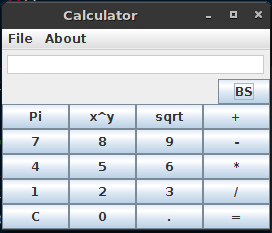
\includegraphics[scale=0.5]{gui.png}
\caption{It should look similar to this}
\end{figure}
You will create an API with JavaDoc which describes a GUI calculator as shown above.
This calculator must be capable of performing addition, subtraction, division, multiplication, and exponential functions on the Real numbers (no Complex values).
The methods for mathematical operations may be used by another program as some later date and should not truncate or round.
Any truncating or rounding must be done after values are passed back to the GUI.

Moreover, the final program should exhibit the following behaviors.
\begin{enumerate}
	\item It should compile.
	\item The API should be written in such a way that code reuse is simple.
	\item The API should be well-documented (if you fill out the JavaDoc correctly you will have done this).
	\item Code should be self-documenting, do not enter comments saying what a switch statement is doing.
	Commenting explains blocks of code.
	If you have to read snippets from multiple classes to understand what a section of code is doing put a comment.
	\item The implementation should take advantage of Java library methods. You may only use the Java standard library.
\end{enumerate}

\section{Part 1: Designing the API}
Design the MathMethods API with which your calculator will interface.
Essentially, \verb|MathMethods.java| is the container for all mathematical operations that the calculator will perform.
It consists entirely of static methods and has no global variables.
Furthermore, each of the methods in MathMethods must return a double.
MathMethods JavaDoc must make mention of when it will throw exceptions due to the operation requested, e.g square root of a negative number.

\section{Part 2: Implementation}
Implement \verb|MathMethods.java|.
Furthermore, you will implement a GUI that will interface with \verb|MathMethods.java|.
This GUI must consist of at least one class, namely \verb|CalcGUI.java|.
You may spread the GUI functions across as many classes as you wish.
The GUI will have a menubar with a File menu and an About menu.
The File menu consists of one item, an exit button.
The About menu consist of one item, an about entry which creates a new window listing the names of the members of the team.
All buttons indicated in Figure 1 above must be present on the calculator.
The calculator may only perform binary operations. 
E.g. ``\verb|2+2=|" is a valid operation, and ``\verb|2+2+2=|" is not.
If a user enters the following ``\verb|2+2=|" and follows this with a ``\verb|+2=|" the calculator should display ``\verb|6|".
The ``\verb|C|" button should clear all input.
The ``\verb|x^y|" button means to compute $x^y$.
The display should display a ``\verb|^|" for both exponentials or roots.
E.g. ``\verb|5^.5|" is $\sqrt{5}$, and ``\verb|5^5|" is $5^{5}$.

\section {Grading}
The primary purpose of this assignment is to demonstrate mastery of writing an API, therefore 60\% of the total grade consists of an evaluation of the API.
The remaining 40\% is in producing a functioning calculator.
The API (skeleton \verb|MathMethods.java| with JavaDoc, A.K.A. Part 1) \textbf{must} be committed to GitHub no later than 11:59pm November 21, 2015.
The source code for Calculator (Part 2) must be committed before class on November 24th.
Deviations from the submitted API must be documented in the JavaDoc of the final code.
Be prepared to see your code displayed, if you write spaghetti everyone will see it.
If your code is completely left justified everyone will see it (and you will lose points on code readability).

\section{Extra Credit}
Implement an algorithm to serve as a proof of concept that $P=NP$.
Add capacity for CalcGUI.java to receive keyboard input.

\end{document}
